\documentclass{proc}

\usepackage{graphicx}

\begin{document}

\title{Perceptually-Optimal Visualization Choice via Just Noticeable Differences}

\author{Lane Harrison}

\maketitle

\section{Introduction}

Much of visualization design remains more art than science \cite{cleveland1982variables}. 
Years of visualization research has led to systems \cite{Mackinlay2007} and guidelines \cite{Zacks1999} that aid the designer in choosing visual representations based on general data characteristics such as dimensionality and data-type.
Yet the designer still faces multiple ambiguous choices for creating visualizations that accurately communicate data.

We believe that experimental methods from vision science can be leveraged to disambiguate visualization choice at a perceptual level.
Vision science has developed experminent methodologies that allow us to determine how much change in a visual scene (e.g. correlation coefficient changes in scatterplots) is required for a typical person to be able to perceive the change.   
Changes exactly large enough to be perceived by a typical person 75\% of the time are referred to as \emph{just-noticeable difference (jnd)}.

Through a series of experiments, we leverage jnd to build perceptual models that describe how different visualization designs (such as scatterplots and parallel coordinates) represent data commonly perceived data characteristics (such as  correlation-coefficient).
If the perceptual models for scatterplots and parallel coordinates differ, our results will demonstrate that a \emph{perceptually-optimal} visualization can be chosen for a given dataset.

\section{One-sentence description}

Leveraging just-noticeable differences to create models of perceived quantities commonly communicated via visualizations, we demonstrate that a perceptually-optimal visualization can be chosen based on data characteristics.

\section{Project Type}

Experiment (crowdsourced)

\section{Audience} 
\begin{quote}
Who is the audience for this project? 
How does it meet their needs? 
What happens if their needs remain unmet?
\end{quote}

If jnd allows us to make perceptually-optimal visualization choices, our results will impact anyone who wants to accurately communicate information via visual representations.
Given a choice between two or more visual representations and a dataset to be shown, this technique will determine which visual representation is optimal for a certain type of perceptual judgment (e.g. correlation coefficient).

This extends the work of Mackinlay et al.'s Show Me work \cite{Mackinlay2007}.
In their system, appropriate visualizations are chosen based on general data characteristics (e.g. dimensionality). 
In our system, however, we will further refine the list of visualizations by calculating commonly perceived values and choosing the optimal visual representation.

\section{Approach}

\begin{figure*}[t]
  \centering
    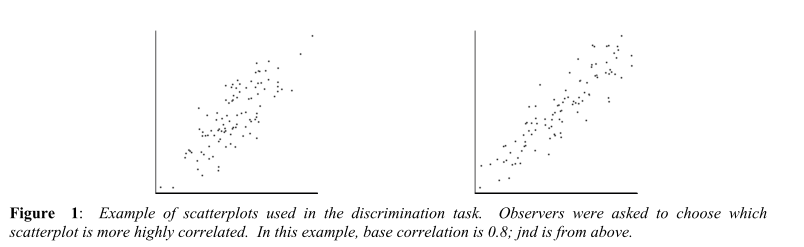
\includegraphics[width=0.9\textwidth]{img/technique}
    \caption{The technique Rensnik used to model how we perceive correlation in scatterplots.}
  \label{fig:technique}
\end{figure*}

\begin{figure}[t]
  \centering
    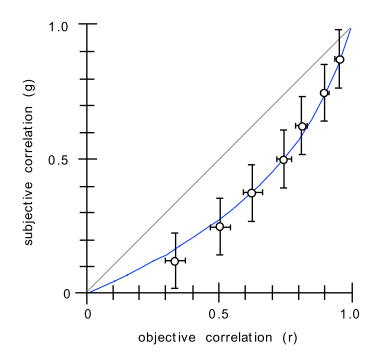
\includegraphics[width=0.5\textwidth]{img/curve}
    \caption{The resulting curve from Rensink's study, showing the perception of correlation (vs. actual correlation) in scatterplots.}
  \label{fig:curve}
\end{figure}


\begin{quote}
What is your approach and why do you think it’s cool and will be successful?
\end{quote}

A few years ago Ron Rensink published ``The Perception of Correlation in Scatterplots'' \cite{Rensink2010}, where he described how jnd can be used to build a model of how well we can distinguish between correlation values.
I believe this technique can be extended to disambiguate between visualization design choices. 
If different visualizations produce different perceptual curves, we can rank them on perceptual accuracy for a given dataset.

The experiment approach Rensink used is illustrated in figure \ref{fig:technique}, and the resulting curve in figure \ref{fig:curve}.

\section{Best-case Impact Statement}
\begin{quote}
In the best-case scenario, what would be the impact statement (conclusion statement) for this project?
\end{quote}

In the best-case, we will show that the perception of correlation in scatterplots and parallel coordinates differ such that if we are given a dataset, we can compute a perceptually-optimal choice between them.
In doing so, we further demonstrate that Rensink's original experiment is a generalizable technique for disambiguating visualization design choices at a perceptual level.

If successful, future experiments using the same technique may be able to answer key questions like how small a visualization can be while still allowing users to accurately perceive important metrics.

\section{Major Milestones}

\begin{itemize}
\item Replicate Rensink's results on Mechanical Turk.
\item Determine a set of visualizations to compare: scatterplots, parallel coordinates, polar representations 2D data, and what else?
\item Pilot to compare scatterplot vs. parellel coordinates correlation judgment.
\item Determine a set of metrics to examine: correlation, outliers(?), data-size(?), width-height(?).
\item Full experiment to compare all chosen visualizations across all chosen metrics.
\end{itemize}

\section{Obstacles}

\subsection{Major obstacles} % (if these fail, the project is over)

\begin{itemize}
\item Replicating Rensink's study on Turk may fail (due to variance in Turker judgments), or at least lead us to a significantly different curve. We would have to consider how our sample populations differ, and whether Turk is truly an appropriate platform for this type of perceptual study.
\item In the pilot (where we compare scatterplots to parallel coordinates) we may find that the curves are too similar (effect size too small) for us to make claims that adapting actually benefits end-users.
\end{itemize}

\subsection{Minor obstacles}

\begin{itemize}
\item The jnd experiment procedure Rensink uses is fairly complex, so it will require a non-trivial amount to setup and test.
\item The original set of visualizations I wanted to compare (scatterplots of varying data size: regular, binned, alpha, jittered) ended up being an imperfect choice since each technique distorts the dataset, which may affect perception. The new set includes: scatterplots and parallel coordinates (horizontal/vertical variations), and polar representations ($\theta, radius$ and $radius, \theta$).
\end{itemize}


\section{Resources Needed}
\begin{quote}
What additional resources do you need to complete this project?
\end{quote}

\begin{itemize}
\item Code to generate datasets for varying correlation-coefficients and data-sizes.
\item Code to make scatterplots similar to the style of Rensink's.
\item A thorough literature review of this space.
\item Someone interested in running web-based experiments, especially with my existing experiment platform (which uses JavaScript, Node.js, d3, and R).
\end{itemize}

\section{5 Related Publications}
\begin{quote}
  List 5 major publications that are most relevant to this project, and how they are related.
\end{quote}

% TODO from Remco: There is a paper in InfoVis this year by Seidlmeir, Melanie Tory, and Munzer that will also be related.

\begin{itemize}
  \item Rensink applied JND to generate a model of how people perceive correlation in scatterplots \cite{Rensink2010}.  \item Mackinlay developed a system that chooses a visualization based on data characteristics \cite{Mackinlay2007}.
  \item Wickham demonstrated a sort of visual t-test, where users had to distinguish between plots of the real data and null plots \cite{Wickham2010}.
  \item Hoffman showed that cartesian representations are superior to polar representations by seeing how well participants could perceive different values between a lineup of charts \cite{Hofmann2012}.
  \item An earlier study from Jing compared how well people can perceive correlation in scatterplots versus parallel coordinates \cite{Li2010}.
\end{itemize}

\section{Define Success}
\begin{quote}
When / How do you know if you have succeeded in this project?
\end{quote}

If, after a pilot, we find that the perceptual curves for correlation in scatterplots are significantly different from those in parallel coordinates, we will have enough evidence to publish a paper that extends the Show Me work in a compelling way.

\bibliographystyle{abbrv}
\bibliography{justNoticeableDiffs}
\end{document}
